\chapter{Introduction}

Das autonome Fahren und die Vernetzung von Fahrzeugen mit Ihrer Umwelt sind zusammen mit der Elektromobilität die meistdiskutierten Themen der Automobilbranche.
Zu Recht: Autonomes Fahren besitzt das Potenzial, im Mobilitätsmarkt völlig neue Strukturen entstehen zu lassen.
\footnote{\url{https://www2.deloitte.com/de/de/pages/consumer-industrial-products/articles/autonomes-fahren-in-deutschland.html} (03/09/2017)}

So ebenfalls die Technische Hochschule Chalmers welche ergänzend zu Volvos “DriveMe” Projekt das Projekt
“CampusShuttle” initiiert hat, “CampusShuttle” ist ein interdisziplinäres Forschungsprojekt der Technischen Hochschule Chalmers und der Universität Göteborg.
Das Projekt ist dabei im ReVeRe (Chalmers Research Vehicle Resource) angesiedelt. Die Vision ist dabei ein selbstfahrendes Auto zwischen den beiden Campus der Technische Hochschule Chalmers.

Dabei soll, im Rahmen des Projekts, das Fahrzeug in verschiedenen Verkehrsszenarien untersucht werden. Der Fokus liegt dabei besonders auf den Stadtverkehr, das Fahrzeug muss dabei nicht
nur in der Lage sein mit anderen Autos zu interagieren, sondern ebenfalls mit Straßenbahnen, Bussen, Fahrrädern aund allen Anderen Verkehrsteilnehmern sicher agieren. 

\section{Ausgangssituation}


\subsection{Test Platform}

\begin{figure}[!ht]
%\begin{center}
\caption{Test Platform Snowfox}
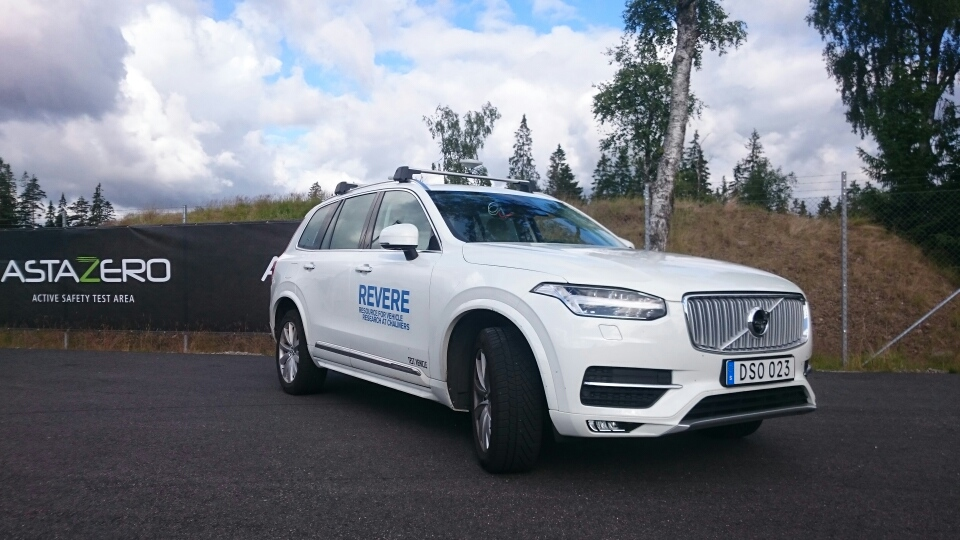
\includegraphics[width=\columnwidth]{bilder/snowfox.jpg}
\label{snowfox}
%\end{center}
\end{figure}

Die in dieser Arbeit genutze Testplatform ist ein Volvo XC90 (2015) SUV, gennate Snowfox (siehe \cref{snowfox}). Diese Testpaltform ist mit vielen Sensoren zur Umfeldwarnehmung ausgestattet.
Dazu zählen fünf Radar Sensoren, rund um das Fahrzeug. Wobei das Front Radar über eine Größere Reichweite verfügt. Sowie eine
Stereo Kamera und ein Velodyne VLP-16 LiDAR. Die Anordnung der Sensoren kann \cref{platform} entnommen werden.


\begin{figure}[!ht]
%\begin{center}
\caption{Snowfox Sensors}
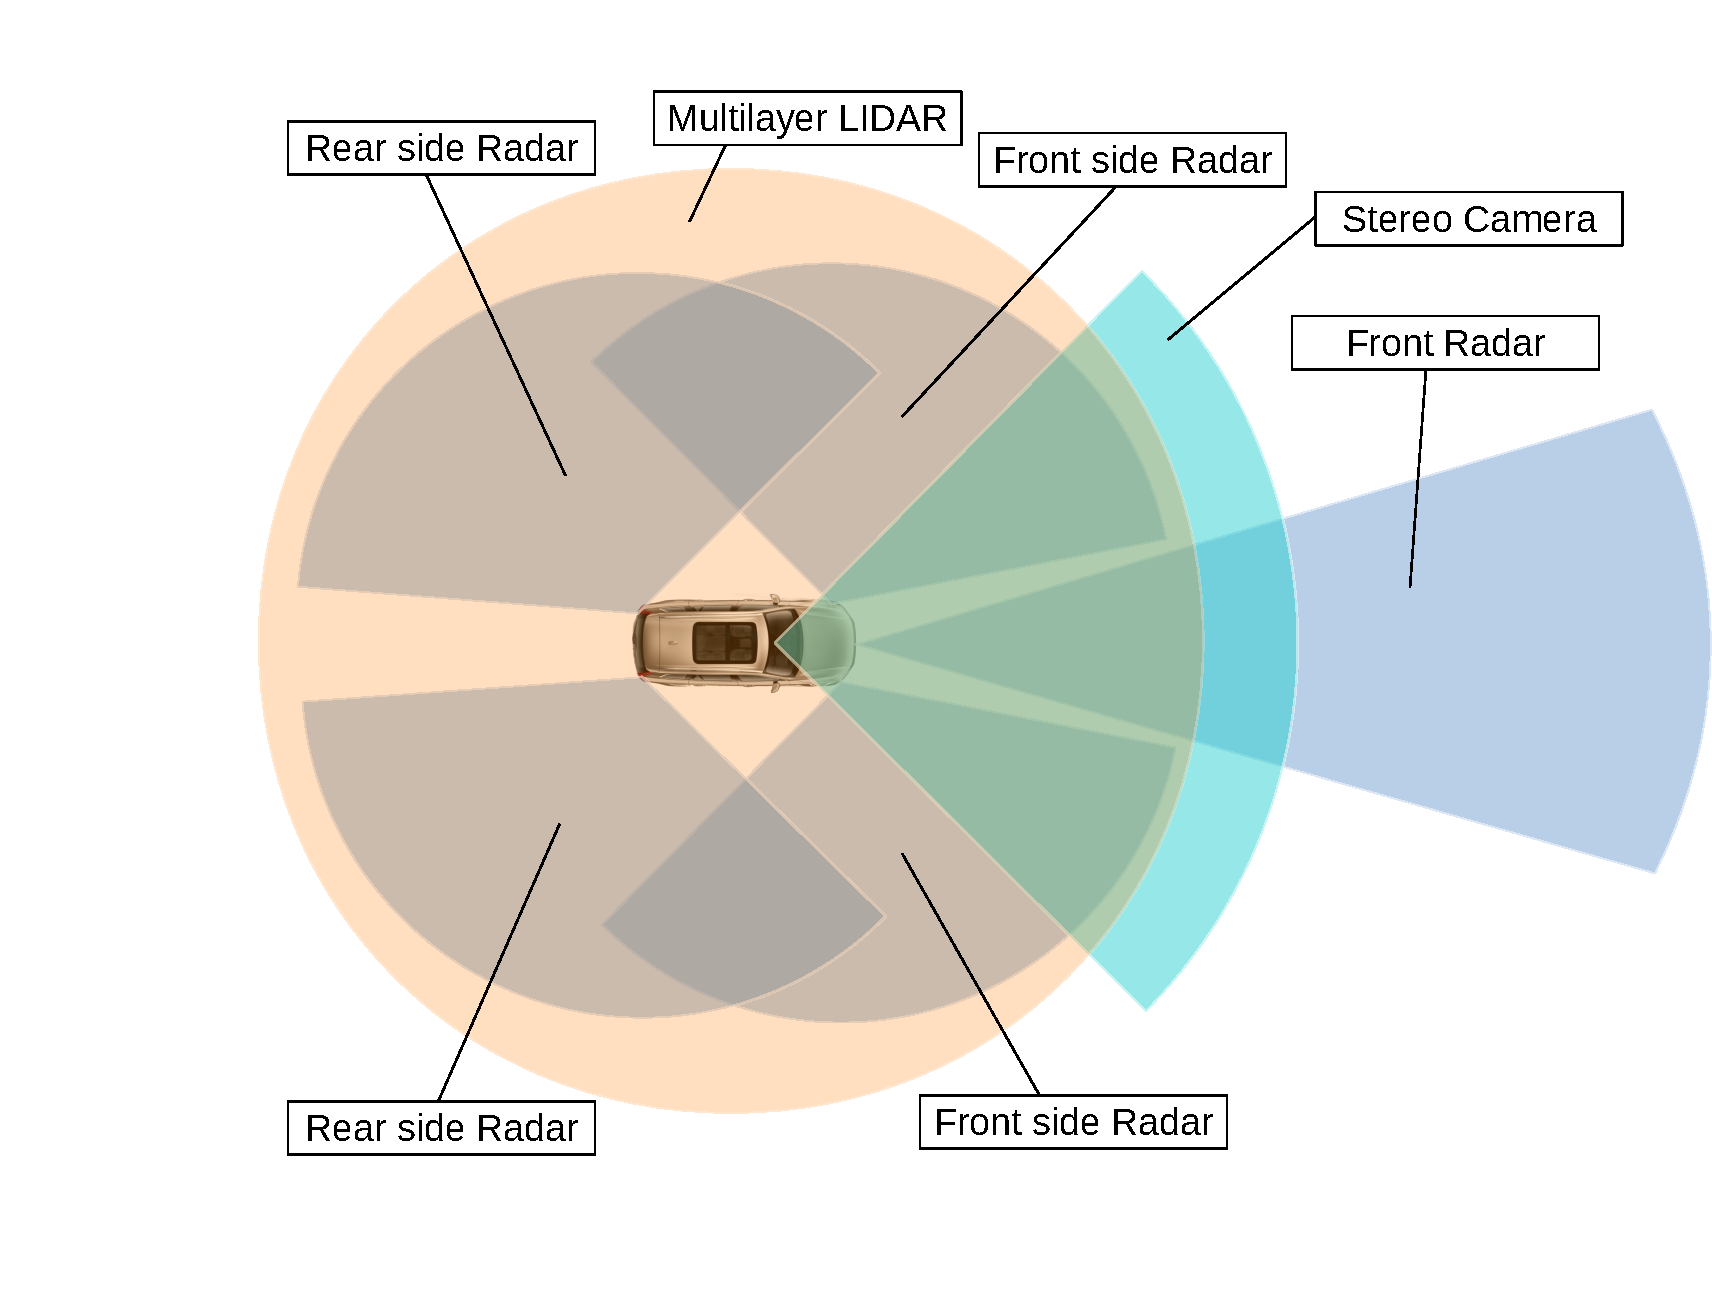
\includegraphics[width=\columnwidth]{sensors.pdf}
\label{platform}
%\end{center}
\end{figure}


Zusätlich zur Serienmäßgigen Fahrzeugsensorik (z.B. Odometer, Interialsensorik) ist im Fahrzeug ein Applanix POS LV verbaut. Zu Zeitpunkt des Verfassens dieser Arbeit war es leider noch nicht möglich auf
die Radarsensoren und die Stereokamera zuzugreifen. Daher werden im folgenden lediglich der Velodyne Lidar und das Applanix System genauer beschrieben.

\subsubsection{Velodyne VLP-16 LiDAR}
\todo{reichweitenanalyse (layer objet mit enbtfernung)}
Der Velodyne VLP-16 ist ein 360 Grad 3D Laserscannermit einer Rotationsgeschwindigkeit von 5 bis 20 Umdrehungen pro Sekunde. Er bietet ein vertikales FOV von 30 Grad, bei 2 Grad Auflösung.
Mit einer Reichweite von 100m kann er einen Umkreis von 200m Durchmesser abdecken. Weiterhin kann der VLP-16 mit dem Applanix POS LV syncronisiert werden, was eine jitterarme Zeimessung ermöglicht.
Eine weiter Funktion des Velodyne Sensors, ist das er auf verschiedene Messimpulse reagieren kann. Durch die Auswertung des letzten Impulses statt des Stärksten Impulses ist es Möglich durch Transparent Objekte zu sehen.
Das ermöglicht uns im späteren Verlauf die Breite des Fahrzeues zu ermitteln, da der Velodyne durch die Glasfenster des Fahrzeues blicken kann.
Bei einer eingestellten Geschwindigkeit von 10Hz liefert der VLP-16 eine Auflösung von 0.2 Grad bei einer Abreichung von +-3cm. Der VLP-16 ist mittig auf dem Dach des XC90 moniert, um eine möglichst hohe Positionierung
zu erreichen, die eine Rundumsicht umd Das Fahrzeug zu erreichen. Zu beachten ist, das diese Ausrichtung für den Sensor denkbar ungünstig ist, da der Sensor ein vertikales
Sichtfeld von -15 bis +15 Grad hat. Dadurch sind nachezu alle messungen über Null grad quasi nutzlos. Der blick auf die Herstellerseite
\footnote{\url{http://velodynelidar.com/vlp-16.html} (03/09/2017)}
verrät, das Der VLP-16 aunteranderem auf die verwendung mit Drohnen hin konstuiert wurde, während der Größere HDL64E
\footnote{\url{http://velodynelidar.com/hdl-64e.html} (03/09/2017)}
explizit für den Urbanen Automotivebereich beworben wird, und über ein Sichtfeld von +2 bis -24.9 Grad verfügt und somit für die Verwendung im
Automotive bereich geeigneter erscheint. Die dabei entstehenden Probleme werden später diskutiert.



\subsubsection{Applanix POS LV}
Das POS LV ist ein kompaktes Positions- und Orientierungssystem. Es Offeriert stabile, zuverlässige und reproduzierbare Positionierungslösungen für landgestützte Fahrzeuganwendungen.
Das POS LV liefert dabei eine Inertialsensork und Odometrie gestützte Positionsmessung mit einer Genauigkeit von bis zu 0.3m (bis zu 0.035m bei verwendung von der der RTK - Korrektur).
Im weiteren Verlauf wird außerdem das vom POS LV gelieferte Heading genutzt, welches eine Genauigkeit von 0.2 Grad liefert. Auch nach ausfall des GPS-Signals kann das POS-LV durch sein
Odeomerter und der Inertialsensork eine Position liefern. Diese wird jedoch über die Zeit schlechter, so das 60Sek nach Ausfall des GPS-Signals nich eine Genauigkeit von 2.51m erwartet
werden kann.\cite{manAP}


\section{Zielsetzung}
Da das Autonome Fahren ein sehr weites, indisziplinäres thema ist, ist es Offensichtlich. das nicht alles in dieser Arbreit abgehandelt werden kann.
Im Rahmen der darpah Chalenge wurden beiteits viele Veröffentlichungen zu diesem Thema erstellet.
Was im rahmen dieser Veröffenticghungten noch nicht berhandelt wurde, sit dei Handhabung von Kreisverkehre, mit atonomen Fahrzeugen.
Ziel dieser Arbeit ist es Daher zu analysieren, welche Sensorausstattung für die beobachtung von Kreisverkehren vonnöten ist, bzw. ob die vorhandenne Sensorausstattung des ReVeRe Testfahrzeuges Snowfox
als ausreichend betrachtet werden kann.

